\hypertarget{st__remove_8c}{
\section{st\_\-remove.c File Reference}
\label{st__remove_8c}\index{st_remove.c@{st\_\-remove.c}}
}


\subsection{Detailed Description}
\begin{Desc}
\item[For internal use only.]
This file contains the implementation of the \hyperlink{group__dbprim__smat_ga24}{\_\-st\_\-remove()} and \hyperlink{group__dbprim__smat_ga14}{st\_\-remove()} functions, which cooperate in removing a sparse matrix entry from the table.\end{Desc}


Definition in file \hyperlink{st__remove_8c-source}{st\_\-remove.c}.

{\tt \#include \char`\"{}dbprim.h\char`\"{}}\par
{\tt \#include \char`\"{}dbprim\_\-int.h\char`\"{}}\par


Include dependency graph for st\_\-remove.c:\begin{figure}[H]
\begin{center}
\leavevmode
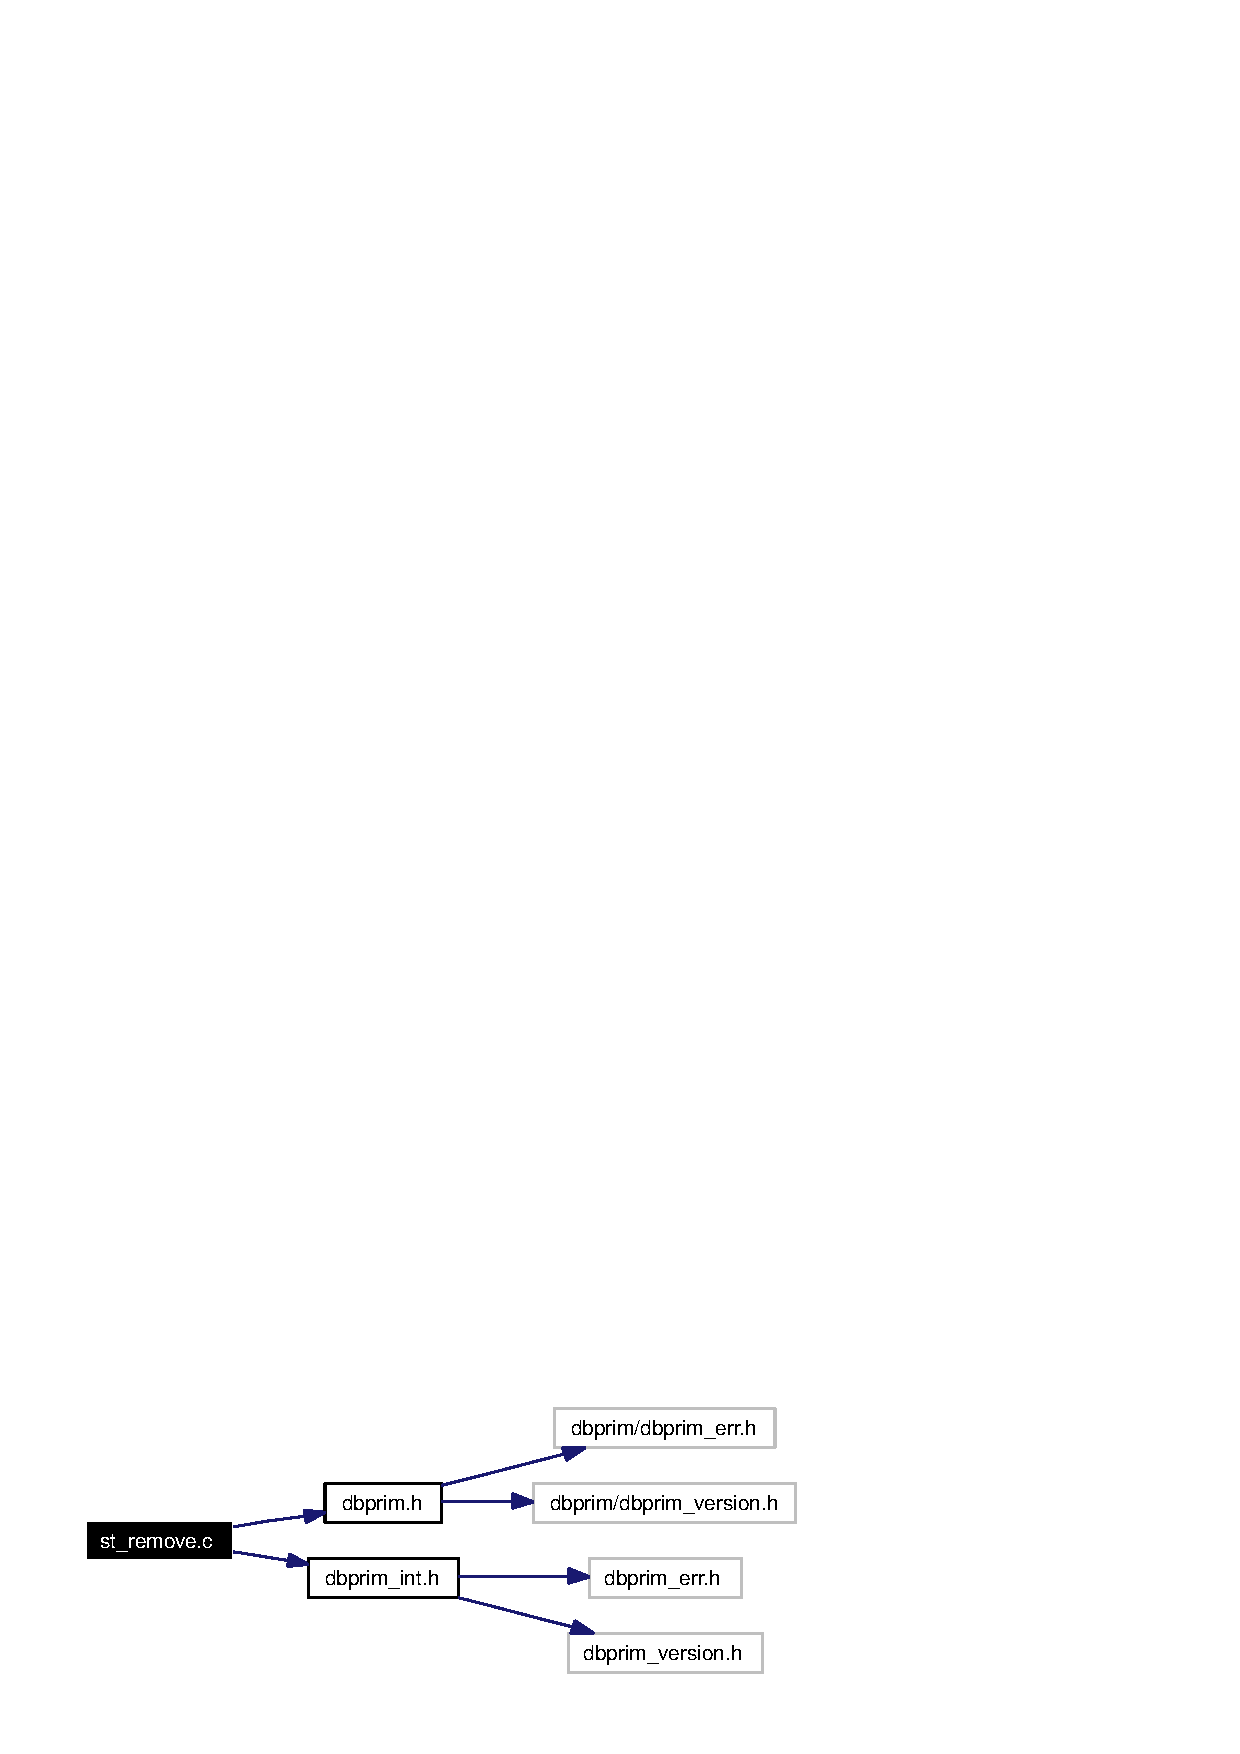
\includegraphics[width=193pt]{st__remove_8c__incl}
\end{center}
\end{figure}
\subsection*{Functions}
\begin{CompactItemize}
\item 
unsigned long \hyperlink{group__dbprim__smat_ga24}{\_\-st\_\-remove} (\hyperlink{struct__smat__table__s}{smat\_\-table\_\-t} $\ast$table, \hyperlink{struct__smat__entry__s}{smat\_\-entry\_\-t} $\ast$entry, unsigned int remflag)
\begin{CompactList}\small\item\em Remove an entry from a sparse matrix (internal). \item\end{CompactList}\item 
unsigned long \hyperlink{group__dbprim__smat_ga14}{st\_\-remove} (\hyperlink{struct__smat__table__s}{smat\_\-table\_\-t} $\ast$table, \hyperlink{struct__smat__entry__s}{smat\_\-entry\_\-t} $\ast$entry)
\begin{CompactList}\small\item\em Remove an entry from a sparse matrix. \item\end{CompactList}\end{CompactItemize}
